% !TEX TS-program = pdflatexmk
% !BIB TS-program = bibtex

\documentclass[12pt, a4paper, twoside]{book}
\usepackage{import}
\subimport{../}{preamble}
\ExecuteBibliographyOptions{articletitle=false}
\standalonetrue
\onehalfspacing
\begin{document}

\begin{singlespace}
{\color{white}
\chapter{Plasmon Interactions in Tip Dimers}}
\label{ch:tip_interactions}
\end{singlespace}

\AddToShipoutPictureBG*{ \AtPageUpperLeft{ \put(0,-240)
{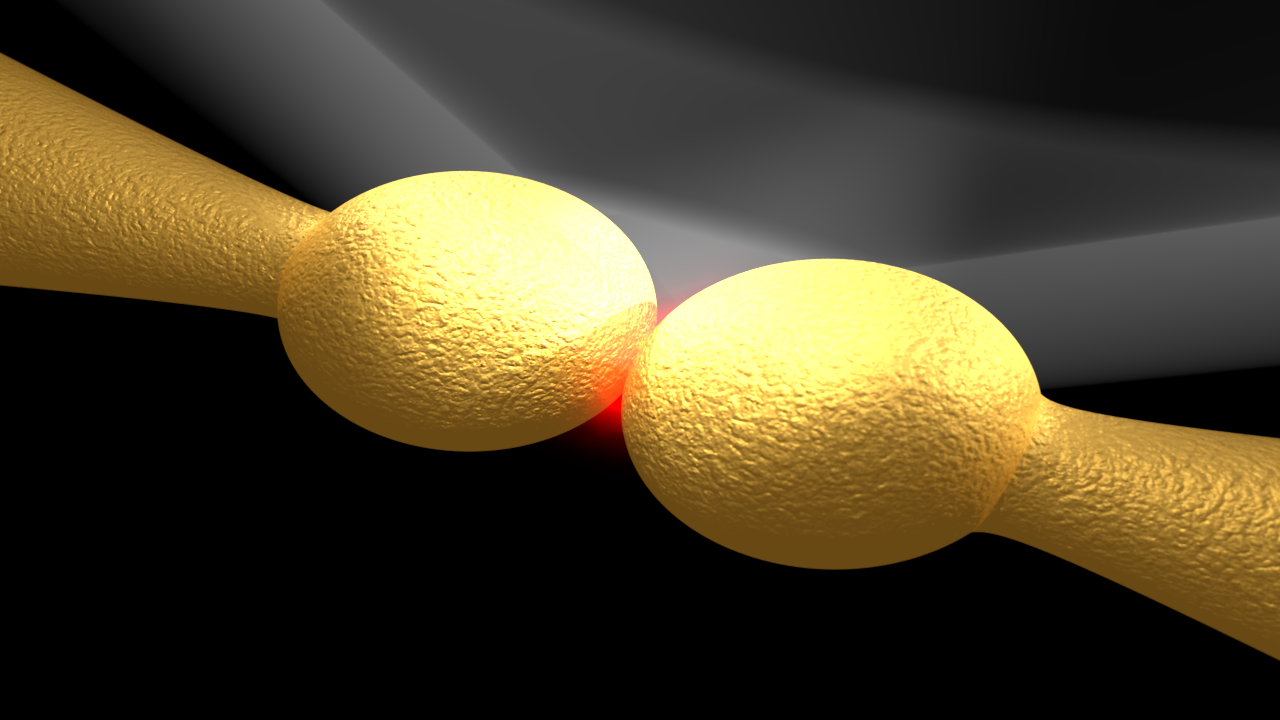
\includegraphics[width=\paperwidth, clip=true, trim=0 80 0 100]{figures/chapter_cover.png}}
}}

The final set of experiments discussed in this thesis are the product of each of the developments from the previous chapters, utilising pairs of tips in the microscope platform to investigate the limits of plasmon coupling. Coupling between different tip morphologies is dynamically investigated to both confirm plasmonic behaviour in tips and increase understanding of the characteristic regimes of plasmon coupling. Through this work an improved interpretation of future results in sub-nm plasmonic gaps can be attained, along with insight into the mechanisms by which \gls{tenom} operates.

\subimport{./}{tip_dimer_interactions}
\subimport{./}{quantum_effects}

\section{Conclusions}

Multiple different combinations of tips in a dimer configuration are used to probe plasmon coupling. Sharp Au tips exhibit no obvious plasmon resonances under far-field illumination and no gap mode coupling is observed with other sharp Au tips or spherical Au tips. This is caused by the lack of antenna modes in the sharp tip geometry.
Plasmons excited at the apex of spherical Au tips, on the other hand, interact and couple to form bonding hybridised modes. The behaviour of these modes is as expected, with similarity to plasmons in AuNP dimers. The inherent asymmetry between the large spherical tip structures leads to a more complex scattering result wherein anti-bonding modes are no longer dark. Their evolution into gap modes is something not previously seen before.

By using such dimer structures the influence of quantum effects, specifically quantum tunnelling, can be probed for sub-nm gaps. The irreproducibility between

While there is little phenomenological dependence on the conduction mechanism it can still be beneficial to identify. In the current experiments there is no solid guarantee, although it is highly likely, that coherent quantum tunnelling is the exact mechanism of charge transfer. To determine this would require tips to be held stably in place while acquiring extra information, such as $dI/dV$ or $dI/dT$. A simpler method would be to compare ambient gaps to molecular spacers. Since molecules have increased tunnelling rates compared to vacuum (or ambient conditions), molecular tunnelling is possible over much larger distances \cite{tan2014}, leading to charge transfer excitation on longer length scales \cite{benz2014}. Exploring this idea of quantum tunnelling vs. molecular tunnelling with conductive molecules during the different phases of making contact is the basis of a future experiment. The idea is also extensible to By coating the tips of a dual-tip plasmonic dimer with dielectric, semiconducting, low-dimensionality or quantum materials, their coupling with plasmons can be directly observed, along with their response to both applied biases and strain.

To conclude, the existence of two distinct regimes of quantum charge transport have been detected in a sub-nm plasmonic cavity. These are:
\begin{itemize}
\item The crossover regime (also known as the tunnelling regime), wherein electrons tunnelling through the barrier screen the capacitive interaction between opposite gap surfaces, reducing plasmon coupling strength and slowing coupling to a halt.
\item The non-local conductive regime, with conduction dictated by the Landauer formula where strong currents form charge transfer plasmons and heavily attenuate and hybridised plasmons are heavily attenuated and blueshifted.
Prior experiments have usually attributed both effects to tunnelling.
\end{itemize}

\ifstandalone
\begin{singlespace}
\fontsize{8pt}{1em}\selectfont
\printbibliography[notcategory=fullcited]
\end{singlespace}
\fi

\end{document}